\documentclass{hipatia}
\usepackage{lipsum}
%Use \DeclareMathOperator para definir novos
% operadores para o modo matemático
\DeclareMathOperator{\sen}{sen}

%Evite numerar teoremas
%Prefira nomeá-los
%Use os ambientes abaixo
\newtheorem*{theorem*}{Teorema}
\newtheorem*{lemma*}{Lema}

% Evite títulos muito longos
\title{Uma Descrição da Gênese do\\ Método Axiomático}
% Se for necessário diminuir a fonte do título 
% para caber no quadro, use
% \title{ \fontsize{28}{28}\selectfont Uma Nova Demonstração do\\  \fontsize{28}{28}\selectfont Teorema de Pitágoras}

% O Subtítulo é o nome da seção da revista
% Deve ser uma palavra de origem grega
\subtitle{História}
\author{Marcelo Papini
}
% A data não é necessária
%\date{October 2023}
% Não se preocupe com a numeração
% das páginas ou com o número da edição

\begin{document}
\setcounter{page}{\historiapage}
\maketitle


A descrição de qualquer fato histórico dependerá da perspectiva adotada pelo narrador. Para   acentuar a possibilidade de se escreverem outras descrições, talvez mais precisas, da gênese do método axiomático, o presente escrito recebeu um título iniciado pelo artigo indefinido ‘\emph{uma}’.
Nada obstante, espera o autor que a presente descrição possa constituir tanto o início de uma reflexão acerca da prática matemática, quanto uma iniciação a um tema extremamente relevante à matemática, à física e à filosofia, qual seja, o \emph{método axiomático}.

%NOTA:  Um par de letras maiúsculas entre parênteses remete às referências bibliográficas  (in fine).



%Sumário

%Antelóquio
%O recurso ao método axiomático
%Referências bibliográficas
%Escritos citados


\section{Antelóquio}

A presença das pirâmides no Egito e de poliedros assemelhados no México atestam que nós, os seres humanos, convivemos  com a geometria há alguns milênios. 

Podemos conjecturar que, inicialmente, os seres humanos houvessem observado diversos fatos geométricos e elaborado hipóteses que os explicassem;  que, depois, houvessem praticado experimentos para verificar as hipóteses pertinentes;  e que, finalmente, houvessem catalogado as hipóteses que tivessem recebido confirmação empírica. 

Apoiando essa conjectura, farei referência apenas ao denominado Papiro de Moscou, ao qual os historiadores atribuíram a data de 1850 a. C.  (época na qual vivia o patriarca Abraão, ainda consoante os historiadores que esmiuçaram o assim chamado \emph{Antigo Testamento} da cultura judaica).

A fim de nos situarmos no tempo histórico, cito o testemunho do escritor helênico Heródoto de Halicarnasso (484 a.C. – 420 d.C.), segundo o qual a geometria nascera no Egito, para atender às exigências de agrimensura impostas aos harpedonaptas\footnote{``Esticador de corda'', agrimensor. (N. do E.)}, obrigados a retraçar os limite dos lotes agrícolas, após as inundações anuais do rio Nilo. 

Os documentos mais abrangentes do saber geométrico egípcio são o papiro Rhind e o papiro de Moscou, que registraram regras para o cálculo da área de algumas figuras planares (como os triângulos, os quadriláteros e o disco) e o volume de alguns corpos (como o cubo, os paralelepípedos, o tronco de cilindro circular e o tronco de pirâmide de base quadrangular).

Do papiro de Moscou, por exemplo, consta a regra para cálculo do volume de uma pirâmide quadrada e truncada, isto é, de uma pirâmide cuja base é um quadrado de lado igual a $B$ e da qual se retirou uma pirâmide a ela semelhante, cuja base fosse um quadrado de lado igual a $C$. O volume desse poliedro é calculado por $$\frac{H}{3}\left(B^2 + BC + C^2\right),$$ onde $H$ indica a altura vertical da pirâmide truncada. \cite[p. 7]{anglin1995}

Segundo uma tradição conservada pelo escritor grego Diógenes Laércio, que viveu pelo século III d.C., a geometria fora transmitida aos gregos por Tales de Mileto, que viajara pelo Egito, relato esse que se deve acolher com cautela pois também de outros intelectuais gregos (como Sólon de Atenas e Demócrito de Abdera) se narram viagens ao Egito, país que fora considerado pelos gregos como ``um repositório de conhecimento invulgar''.  \cite[p. 11]{momigliano1991}

Essa mesma tradição atribui a Tales de Mileto a prova de alguns fatos geométricos mas, na primeira fase evolutiva da matemática grega, a prova consistia em tornar evidente  [ e + vidêre = ver]  ou visível a veracidade de uma sentença. A isso chamava-se \emph{método epagógico}. \cite[p. 127--128]{otte2006}

Segundo o testemunho de Proclo de Constantinopla, para \emph{provar visualmente} (empregando, pois, o método epagógico) a congruência entre os dois triângulos obtidos de um triângulo isósceles, ao se traçar a bissetriz do ângulo cujos lados fossem congruentes, Tales dobrava ao longo dessa bissetriz uma figura concreta de um tal triângulo. 

Ainda segundo Proclo, dobrando a figura concreta de um disco ao longo de um qualquer diâmetro, Tales teria provado visualmente que todo diâmetro de um disco o divide em duas partes congruentes.  \cite[p. 25]{coolidge1940}\cite[p. 25]{mosterin1984}

Desse modo, Tales parece haver vislumbrado a primazia do \emph{conceito de congruência}, que desempenharia papel decisivo no pensamento geométrico. 

Na fase evolutiva seguinte, a ênfase foi transferida para o \emph{método apagógico}, que consistia em se fornecer um argumento, construído mediante o encadeamento de proposições, o qual sustentasse a sentença considerada. Conjuntamente, esses dois métodos indicam dois aspectos da atividade intelectual: o aspecto perceptual e o aspecto conceitual.  \cite[p. 121]{otte2006}

Ainda não se pôde precisar quando o saber geométrico se converteu em um corpo de proposições sequencialmente articuladas. Atribui-se à escola jônica e à escola pitagórica a substituição dos enunciados de fatos empíricos insulados por cadeias de proposições, na qual cada proposição ocupasse um lugar definido e fosse inferida das proposições que a antecedessem. Dessa fase histórica resta-nos apenas um fragmento, os \emph{Elementos}, do filósofo jônico Hipócrates de Quios (\emph{circa} 430 a.C.).  \cite[p. 120]{kagan1986}\cite[p. 1]{sommerville1958}\cite[p. 39--40]{struik1987}

Nesses \emph{Elementos} de Hipócrates, os juízos se classificavam em dois tipos, conforme a sua veracidade se instituísse empírica ou dedutivamente.  \cite[p. 12]{smogorzhevski1976}

Mas podemos supor que essa conversão do saber geométrico, de um corpo de regras empíricas em um corpo de juízos sequencialmente articulados, tenha sido contemporânea com a instituição da pólis na cultura helênica e com a concomitante ascensão da palavra, o \emph{logos}, a ferramenta de poder: ``A arte política é essencialmente um exercício da linguagem; e o \emph{logos}, na origem, toma consciência de si mesmo, de suas regras, de sua eficácia, através de sua função política.'' \cite[p. 17]{chatelet1994}\cite[p. 35]{vernant1984}

Para ensinar a técnica de uso da palavra, surgiram os sofistas, mestres da retórica, e, dentre eles, o \emph{arquissofista} Sócrates (apelido dado pelo poeta cômico Aristófanes).  Platão, pensador helênico do quarto século a.C., no diálogo Laques, atribuiu a Sócrates a invenção ``de uma coisa nova que, vinte e quatro séculos depois, seria denominada \emph{o conceito}''. \cite[p. 20]{chatelet1994}

A discussão de temas matemáticos por filósofos da cultura helênica, na época em que viveu Platão, constitui um fato surpreendente. Em seu diálogo \emph{Menon}, Platão narra que seu antecessor, Sócrates, passeando com um jovem, indagou como se poderia obter um quadrado cuja área fosse o dobro da área do quadrado cujos lados exibissem o comprimento $L$. Diante da resposta de que seria suficiente dobrar o comprimento dos lados  ($2L$), Sócrates recorreu a um diagrama desenhado na areia com uma bengala, para mostrar que, dobrando o comprimento dos lados,  produziríamos um quadrado cuja área equivaleria a quatro vezes a área do quadrado considerado inicialmente  ($4L^2$). (Usando o nosso contemporâneo \emph{modus loquendi}, podemos dizer que a área de um quadrado \emph{não seja função linear} do comprimento de seus lados.)

E, recorrendo a outro diagrama, Sócrates demonstrou que, para obtermos um quadrado cuja área fosse o dobro da área do quadrado considerado, seria suficiente tomar como lado desse segundo quadrado uma das diagonais do primeiro quadrado.

Se me perguntassem qual foi o intento de Platão nesse diálogo, eu diria que ele nos advertia de que nem sempre nossas primeiras intuições sejam verdadeiras. 

Por honestidade intelectual, cabe-me revelar que muitos comentadores sustentam que Platão estivesse argumentando em favor da \emph{anamnese}  (doutrina cuja exposição é impertinente ao tema do presente escrito). Contudo, é estimulante perceber que, recentemente, o método didático adotado por Sócrates no citado diálogo, método esse denominado \emph{maiêutica socrática}, vem sendo propugnado como ferramenta propedêutica da matemática. \cite[p. 8]{winter1989}

De qualquer modo, citei esse passo da obra de Platão, para mostrar que, naquela época, discutir argumentos geométricos não fosse alheio à prática filosófica, sugerindo que a catalogação das hipóteses empiricamente confirmadas  (catalogação essa que conjecturei no início deste escrito)  já se encontrasse em uma fase avançada.

O citado modo de se articularem proposições apresenta dois aspectos. Em primeiro lugar, cada teorema, por se deduzir das proposições anteriores, se liberava de qualquer verificação empírica, reservada apenas às proposições primeiras, que, inicialmente, se escolheriam por sua evidência e por sua simplicidade. Em segundo lugar, a possibilidade de se obterem enunciados de proposições geométricas, independentemente da comprovação experimental, provocou um progresso muito mais rápido e permitiu que o acervo de enunciados se enriquecesse ao ponto de discorrer sobre noções cuja elaboração não se efetuaria no nível puramente empírico e cuja verificação seria inexequível empiricamente.  \cite[p. 120]{kagan1986}\cite[p. 12]{smogorzhevski1976}  

Essa ausência de verificação empírica exigiu que o modo de argumentação fosse adequadamente sistematizado, sistematização essa que, talvez, fosse intensamente discutida na Academia de Platão de Atenas.

Com efeito, conta-se que, após escrever o diálogo \emph{Protágoras}, no qual se opõem as opiniões desse filósofo e as de Sócrates, Platão se sentiu insatisfeito em apenas confrontar os supostos saberes de sofistas e de políticos e desejou encontrar base sólida para fundamentar o seu pensamento. Parecendo-lhe que os geômetras teriam algo por lhe oferecer, Platão viajou a Cirene (na costa africana), onde assistiu às preleções de Teodoro, o qual perseguia a classificação dos quadrados, conforme a comensurabilidade entre a grandeza do lado e a unidade. Em seguida, foi à Itália, onde estudou com Arquitas de Tarento, criador da teoria das médias proporcionais (a qual seria, posteriormente, exposta no tomo VIII dos \emph{Elementos} de Euclides de Alexandria).  \cite[p. 103]{laercio1988}\cite[p. 170, 182]{mosterin1984}\cite[p. 209]{russell1945} 

Regressando a Atenas, Platão fundou a Academia, onde se cultivaria a matemática, em oposição à escola de Isócrates, cujo ensino era dirigido à política. Na Academia ensinou o geômetra Teeteto de Atenas, que concluíra o estudo dos números irracionais desenvolvido por Teodoro de Cirene, descobrira o octaedro e o icosaedro e mostrara existirem apenas cinco sólidos regulares. (Essas teorias seriam, posteriormente, explicadas nos tomos X e XIII dos Elementos de Euclides.)  \cite[ p. 64]{aaboe1984}\cite[p. 172, 188]{mosterin1984}\cite[p. 147]{russell1945}

O asserto de que Teodoro houvesse descoberto dois dos cinco poliedros regulares deve ser lido \emph{cum grano salis}. Sabe-se que diversas substâncias se apresentam naturalmente em formas cristalinas, das quais algumas são regulares, como o hexaedro. Babor \& Ibarz ensinam que o cloreto de sódio e o fluoreto de cálcio ocorrem na forma de hexaedro regular. \cite[p. 84]{babor1960}

Por sua vez, do sulfeto de ferro (ou pirita, $\mathrm{FeS}_2$), que se apresenta como dodecaedro, havia jazidas na Magna Grécia (sul da Itália).  \cite[p. 41--42]{struik1987}
Isso nos leva a buscar a origem dos ‘sólidos platônicos’ na mineração primitiva. 

Também na Academia professou aulas o notável geômetra Eudoxo de Cnido, que elevou o nível de rigor nas demonstrações, criou a teoria das proporções (tomo V dos \emph{Elementos} de Euclides) e elaborou o método de exaustão (tomo XII dos \emph{Elementos}), baseado em um critério que permitiu refutar as aporias de Zenão de Élea.   \cite[p. 64]{aaboe1984}\cite[p. 175]{mosterin1984}

Vale lembrar que as supostas antinomias indicadas por Zenão de Élea  (bem como as discussões conduzidas por diversos sofistas)  lançavam dúvida acerca da adequação do raciocínio, expresso na linguagem, como ferramenta para se atingir a verdade. Tais discussões constituíam uma ``arma dialética e destrutiva'', que ``conturbava as primeiras especulações dos matemáticos acerca das relações no espaço ou no tempo, proibindo ao espírito humano alcançar a inteligência de uma quantidade pela medida das suas partes''. \cite[p. 154]{brunschvicg1972} 

No caso do argumento da dicotomia, por exemplo, Zenão afirmava que, a fim de transpor um percurso de comprimento $L$, o móvel teria de transpor, antes, a metade desse percurso (de comprimento $L/2$) e, antes de transpor a sua metade, teria de transpor a sua quarta parte (de comprimento $L/4$) etc. Daí pretendia concluir Zenão pela impossibilidade do movimento, conclusão essa constantemente contestada pela experiência. Ora, diriam os adeptos de Zenão, se a razão mostra que o movimento não existe e a experiência mostra que essa ilação é falsa, então a razão não é confiável.

Mas esse argumento de Zenão se reduzia, em última instância, à suposição de que fosse infinita a soma da série $1/2 + 1/4 + 1/8 + \cdots$, opinião que, por suas consequências, pode causar admiração mas que é \emph{facilmente confutável}. 

Aliás, não é tão raro que alguns pensadores se ancorem em um erro para construir um argumento. Ainda no século XVII, o argumento de Zenão era retomado por diversos críticos da matemática, consoante informa Brunschvicg.  \cite[p. 154]{brunschvicg1972}  

E Russell  denunciou que os adeptos de Georg Hegel e os prosélitos de Henri Bergson, respectivamente, sob a égide da razão e da intuição, veneraram prejuízos defendidos por ignorantes da matemática. \cite{russell1945}

A impressão profunda que a matemática causou a Platão é patente no seu asserto de que é ignominioso o desconhecimento da teoria das grandezas incomensuráveis, mal merecendo o qualificativo de humano aquele que a ignora. Também é sintomática a interdição ao ingresso na Academia daqueles que não se interessassem pela geometria. \cite[p. 21]{lanczos1970}\cite[p. 209--210]{russell1945}  


\section{O recurso ao método axiomático}

É possível que a Lógica houvesse nascido da observação, na Academia platônica, do método usado pelos matemáticos Arquitas, Teeteto e Eudoxo nas discussões acerca das propriedades aritméticas e geométricas. Assim, a Lógica teria origem empírica, entendendo-se por empírica qualquer atividade associada à experimentação. No caso vertente, experimentavam-se argumentos dedutivos.

Essa MINHA opinião não parece destoar do que assere Bruno Latour no seguinte excerto:
\begin{quote}
    Os vocábulos \emph{apodixe} e \emph{epidixe} têm quase a mesma raiz etimológica e, por muito séculos, eram completamente indistinguíveis. Foram somente os filósofos platonicistas que, conformando sua linguagem pelo efeito persuasivo que resultava das demonstrações geométricas, introduziram na filosofia uma diferenciação radical entre um modo de se convencer (mediante demonstrações rigorosas), a \emph{apodixe}, e outro modo que dependia de floreados de retórica, de sofística, de poética, da imaginação e de artifícios políticos, a \emph{epidixe}. \cite[p. 445--446]{latour2008}
\end{quote}

Atribui-se a Aristóteles de Estagira, na obra \emph{Primeiros Analíticos}, a sistematização inicial dos rudimentos da Lógica, qual seja, a teoria dos silogismos. Embora, com o descenso dos tempos, a construção da Lógica tenha sofrido profunda modificação, parece ser permanente a ideia constitutiva, já patente nos escritos do Estagirita, de que a Lógica (formal) se ocupe das regras que permitem extraírem-se conclusões válidas, independentemente do conteúdo semântico das premissas. Note-se que o vocábulo Lógica, na acepção da doutrina discutida por Aristóteles ao longo de sua obra \emph{Organon} (reunião de escritos produzidos em diferentes datas), foi empregada, pela primeira vez, por Alexandro de Afrodísias, no começo do século III d.C. 

Na obra \emph{Segundos Analíticos}, Aristóteles, possivelmente baseado no modelo da geometria o qual lhe era contemporâneo, definiu uma ciência dedutiva, notando que é impossível tanto definir tudo, quanto demonstrar tudo  (pois uma tentamento de fazê-lo conduziria a um regresso \emph{ad infinitum}). Por isso, esse autor helênico escolheu como primitivos os conceitos que dispensam definição  (por ser patente o seu significado)  e os juízos que prescindem de demonstração  (por ser patente a sua veracidade). 

Assim, segundo a visão do Estagirita, uma ciência dedutiva é um sistema $S$ de termos e de enunciados tais, que
\begin{enumerate}
    \item Todos os enunciados de $S$ se referem a um mesmo domínio de objetos reais.
    \item Todos os enunciados de $S$ são verdadeiros.   
      
\item Pertencem a $S$ todos os enunciados que sejam consequência lógica de enunciados de $S$.
\item Existe em $S$ um conjunto finito de termos cujo significado prescinde de explicação e mediante os quais se podem definir todos os outros termos de $S$. (\emph{Conceitos primitivos}.) 
\item Existe em $S$ um conjunto finito de enunciados cuja veracidade é evidente e dos quais decorram todos os outros enunciados de $S$.  (\emph{Proposições primitivas}.)   \cite{costa1994}
\end{enumerate}

Afirmam os estudiosos da matemática helênica que os Elementos de Euclides  (século III a.C.)  tenham sido redigidos consoante a formulação descrita pelo Estagirita. Por exemplo, Evert Beth declarou que ``a matemática clássica constitui o exemplo por excelência, e talvez o único exemplo, de uma teoria dedutiva, consoante a teoria das ciências de Aristóteles''. \cite{beth1955}

A obra de Euclides é iniciada com uma lista de definições, das quais a primeira consiste em asseverar que ``\emph{um ponto é aquilo que não tem partes}''. Essas definições não são logicamente operativas. Constituem apenas elucidações vagas, nas quais termos usados na enunciação dos postulados e dos teoremas são parcialmente explicados mediante termos que não pertencem ao sistema.

Alguns críticos supõem que, ao propor tais definições, Euclides estivesse explicitamente declarando que, na composição dos \emph{Elementos}, não seria adotada a concepção atômica esposada por Demócrito de Abdera. 

Após as definições, Euclides expôs alguns enunciados primitivos, classificando-os em \emph{axiomas} e \emph{etemas}  (termo grego equivalente ao termo latino \emph{postulatus}). Os axiomas parecem tratar de fatos gerais  (são juízos concernentes a qualquer espécie de grandeza), enquanto os postulados se referem a fatos específicos da ciência vertente  (são juízos cuja veracidade é proposta no corpo do texto). Essa distinção entre os significados dos dois vocábulos esmaeceu ao longo dos séculos.

Eis os %oito
cinco axiomas e os cinco postulados de Euclides: 

Axiomas
\begin{enumerate}
    \item 
  Coisas iguais a uma coisa são iguais entre si.
\item  Se a coisas iguais foram somadas coisas iguais, as somas também serão iguais.
\item  Se de coisas iguais forem subtraídas coisas iguais, os restos também serão iguais.
%\item  E se coisas iguais forem somadas a coisas desiguais, as somas serão desiguais.
%\item  E coisas iguais ao dobro da mesma coisa são iguais entre si. 
%\item  E as metades da mesma coisa são iguais entre si. 
\item  Coisas que coincidem entre si são iguais. 
\item O todo é maior que suas partes.
\end{enumerate}

Postulados

\begin{enumerate}
\item    Fique postulado traçar uma reta a partir de todo ponto até todo ponto.
\item    Também prolongar uma reta limitada, continuamente, sobre uma reta.
\item    E, com todo centro e distância, descrever um círculo.
\item     E serem iguais entre si todos os ângulos retos.
\item    E, caso uma reta, caindo sobre duas retas, faça os ângulos interiores e do mesmo lado menores do que dois retos, sendo prolongadas as duas retas, ilimitadamente, encontrarem-se no lado do qual estão os menores do que dois retos.
\end{enumerate}

Existe um claro dissenso entre os escoliastas acerca da credibilidade das versões disponíveis dos Elementos. 

Consoante Vincenzo De Risi, 
\begin{quote}
os treze livros dos \emph{Elementos} de Euclides, provavelmente, foram escritos no terceiro século a.C., coligindo materiais de uma tradição matemática mais antiga, e, certamente, sofreram diversas mudanças já na era helenística. Muitos séculos depois, o matemátio Theon de Alexandria (quarto século da era cristã) preparou um edição dos Elementos, a qual teria enorme importância na tradição subsequente do texto. Contudo, as cópias mais antigas disponíveis dos Elementos são cópias de manuscritos bizantinos que remontam ao início do século nono. Manuscritos gregos posteriores circularam entre os eruditos durante o Renascimento e, de fato, constituíram o texto grego para as primeiras edições do escrito de Euclides no mundo moderno.  \cite[p.  595]{risi2016}
\end{quote}


Euclides foi particularmente feliz na formulação do seu quinto postulado (ou quinto etema), o qual, enunciado apenas após o teorema I.27, incomodou longamente os matemáticos subsequentes que se detiveram no exame do ordenamento das proposições. Se houvesse apresentado o quinto postulado anteriormente, Euclides teria simplificado alguns argumentos.

Desde o século I a.C., houve tentamentos em se demonstrar o quinto etema de Euclides, os quais repousavam na admissão (tácita ou explícita) de outros postulados. \cite[p. 2]{bonola1906}

Proclo de Constantinopla (comentador do século V d.C.) sustentava dever o quinto postulado de Euclides ser excluído do elenco de postulados, por ser um teorema (cuja demonstração já teria sido tentada por Ptolemeu).  \cite[p. 68]{coolidge1940}

Por outro lado, a  proposição I.27 dos Elementos é o teorema: ``São paralelas duas retas que, intersecadas por uma terceira, formam com essa última ângulos alternos internos suplementares.''

Intensamente perplexo, Proclo perguntava: ``Pode uma proposição ser um teorema e, simultaneamente, pode sua recíproca ser um postulado?''

Dúvidas dessa natureza suscitaram a busca de um critério que permitisse reconhecer se um enunciado apresentasse o caráter de axioma ou de teorema. Foi no contexto dessas discussões que nasceu a noção de \emph{postulados independentes}, isto é, de postulados que integram um sistema que empobrece, se algum dos postulados for excluído. Isso significa que nenhum dos postulados pode ser deduzido dos outros. A um enunciado dedutível dos outros chamamos \emph{postulado redundante}.  A um sistema axiomático composto apenas de postulados independentes chamamos \emph{sistema irredutível}.  \cite[p. 131]{moise1963}\cite[p. 985]{scanlan1988}

Note-se que, ao longo de toda essa discussão, não se pôs em dúvida a veracidade do sistema geométrico erigido por Euclides de Alexandria. O questionamento incidia apenas sobre o modo de se escolherem os postulados. 

Mas, com o passar dos séculos, também se passou a suspeitar que fosse possível construírem-se outros sistemas de axiomas geométricos. 

Na verdade, um tal sistema já fora construído por Menelaus (\emph{circa} 100 d.C.), ao estudar a geometria sobre a superfície esférica. Talvez por tal esfera estar imersa no espaço usualmente descrito pelo sistema euclidiano, não se reconheceu que a geometria intrínseca da esfera constituísse um novo modelo de geometria planar.  \cite[p. 57]{struik1987} 

Dentre os tentamentos em se demonstrar o quinto postulado de Euclides o mais notável foi conduzido por Gerolamo Saccheri, que recorreu ao método denominado \emph{reductio ad absurdum}, aplicado à figura obtida, quando se traçam, pelas extremidades de um segmento de reta $AB$, as perpendiculares $r$ e $s$ e, sobre essas retas, no mesmo semiplano, se marcam os segmentos congruentes $AC$ e $BD$. Saccheri mostrou (recorrendo aos critérios de congruência de triângulos) que são congruentes os ângulos $\angle ACD$ e $\angle BDC$ e considerou os três casos: 
(a)  Ambos os ângulos são agudos. 
(b)  Ambos os ângulos são retos. 
(c)  Ambos os ângulos são obtusos.

Em seguida, Saccheri mostrou que a segunda hipótese implicasse o postulado de Euclides e tentou mostrar que as duas outras hipóteses fossem falsas. Na verdade, seu tentamento em mostrar a falsidade das duas outras hipóteses produziu enunciados de um sistema geométrico distinto do euclidiano, os quais Saccheri, falaciosa mas indolosamente, supôs serem impossíveis.  \cite[p. 182]{kneebone1963}

Coube a Nikolai Lobachevski a glória de haver composto, em 1826, o primeiro estudo explícito de um sistema geométrico distinto do adotado até então\footnote{
Essa glória é compartilhada com o matemático húngaro
János Bolyai, que também desenvolveu, de maneira independente, um sistema não euclidiano em meados da década de 1820, o qual foi publicado em 1831.  
(N. do E.)}. Lobachevski iniciou seu trabalho, recorrendo também à \emph{reductio ad absurdum}, pelo tentamento em demonstrar o enunciado que Euclides expusera como o quinto postulado, mediante o uso explícito do argumento seguinte: Sejam $A$ o quinto postulado de Euclides e $B$ um juízo que se obtém a partir de $\neg A$  (a \emph{negação} de A). Se $B$ for incompatível com o sistema axiomático que se obtém, excluindo-se o quinto postulado do sistema de Euclides, então também $\neg A$ será incompatível com tal sistema. Isso comprovaria $A$.   \cite[p. 29]{bachelard1934}\cite[p. 388]{kneale}\cite[p. 13--14]{smogorzhevski1976}      

Para sua surpresa, Lobachevski não obteve nenhum enunciado que contradissesse o sistema geométrico de Euclides. Isso sugeria que o quinto postulado fosse efetivamente um enunciado independente dos demais enunciados do sistema euclidiano. 

Assim, Lobachevski foi precursor do método de verificação da independência de um enunciado $\alpha$ relativamente a um sistema axiomático $\Gamma$. Tal método consiste em exibirem-se modelos de estruturas que satisfaçam ou a $\Gamma\cup\{\alpha\}$ ou a $\Gamma\cup\{\neg\alpha\}$. 


Em oposição ao sistema de Euclides, o sistema axiomático obtido pela substituição do quinto postulado pelo asserto de que existem diversas retas paralelas a uma mesma reta por um mesmo ponto foi denominado \emph{não euclidiano} por Carl Gauss, em uma carta de 8 de novembro de 1824.  \cite[p. 39]{barbosa1995} 

Incumbe notar que os qualificativos anti-euclidiano e não-euclidiano, empregados, inicialmente, por Gauss para designar sistemas de postulados geométricos distintos do sistema euclidiano, não têm caráter matemático mas tão somente sabor histórico. De fato, como até então somente se conhecesse o sistema euclidiano  (que então era descrito simplesmente como \emph{a geometria}), os novos sistemas receberam tais qualificativos por oposição ao sistema geométrico já estabelecido (e, desde então, o sistema previamente instituído também recebeu o qualificativo de \emph{euclidiano}). 

Mas tal episódio constituiu apenas uma vicissitude ou uma contingência histórica e não um critério classificativo. Creio que, já em 1871, Felix Klein estava fortemente convencido disso pois, nesse ano, escreveu sobre ``\emph{a assim denominada geometria não euclidiana}'' [\emph{die sogenannte nicht-euklidische Geometrie}].  \cite[p. 67]{bonola1906}\cite[p. 214]{yaglom}  

Contudo, o problema da consistência não fora resolvido. Bolyai e Lobachevski, efetivamente, não encontraram contradições em seus incursos por esse novo domínio. Mas nada certificava que, no futuro, não se manifestassem tais contradições. E assim foi suscitado \emph{o problema da consistência}.  \cite[p.  388]{kneale}  

Baseando-se em uma memória de Eugenio Beltrami, Jules Houël (1869-1870) ofereceria a primeira solução ao problema da consistência do sistema de Lobachevski, construindo-lhe um modelo euclidiano. Com efeito, Beltrami havia mostrado que os teoremas obtidos por Lobachevski eram verificados em uma superfície de curvatura constante negativa.  \cite[p. 320--321]{kagan1986}\cite[p. 32--33]{carmo1988}  

Nessas condições, a qualquer contradição na geometria de Lobachevski corresponderia uma contradição na geometria de Euclides. E assim também mostrou que não se poderia provar o quinto postulado de Euclides, já que tal prova implicaria a falsidade do postulado correspondente de Lobachevski. A esse tipo de solução do problema da consistência chamou-se \emph{prova relativa de consistência}.  \cite[p. 388]{kneale}\cite[p. 325]{fraenkel1963}

A segunda solução seria dada por Felix Klein, em 1871, ao  mostrar que a geometria de Bolyai e Lobachevski poderia ser considerada como uma geometria projetiva com uma métrica de Cayley. Assim, ``se houvesse incongruências na geometria de Bolyai e Lobachevski, também se poderiam encontrar incongruências na geometria projetiva e poucos matemáticos estavam dispostos a admitir tal heresia''. \cite[p. 178]{struik1987}  

Também o argumento de Klein constituiu uma prova relativa de consistência da geometria de Bolyai e Lobachevski.

Impuseram-se, assim, dois novos problemas: a prova de consistência da geometria euclidiana e a prova de consistência da geometria projetiva. Ambos esses problemas podem resumir-se nas palavras atribuídas a Henri Poincaré: ``Para preservar dos lobos um rebanho, não é suficiente guardá-lo no redil; é necessário verificar, além disso, que, no redil, não existe lobo algum.''  \cite[p. 59]{babini1974}

Um avanço na solução desses novos problemas foi obtido por Moritz Pasch que, nas \emph{Preleções sobre a nova geometria [Vorlesungen über neuere Geometrie (1882)]}, mediante a escolha judiciosa dos conceitos e dos juízos primitivos, tentou ``fundar empiricamente a geometria''. \cite[p. 151]{pasch1924} 

Consoante a interpretação por da Costa, Pasch ``apresentou uma sistematização precisa da geometria comum como disciplina física''.  \cite[p. 193]{costa1994}

Nessa obra, assim se exprimia Moritz Pasch: 
\begin{quote}   
Se quisermos que a geometria seja verdadeiramente dedutiva, o processo dedutivo deverá ser totalmente independente do significado [Sinn] dos conceitos geométricos assim como deverá ser independente das figuras. Somente as relações entre os conceitos geométricos que houverem sido explicitadas nas proposições e nas definições adotadas deverão ser consideradas. É verdade que, no curso de uma dedução, seja permitido e útil conservar no espírito a referência [\emph{Bedeutung}] dos conceitos geométricos empregados mas isso não é absolutamente necessário.  
\cite[\emph{apud}, p. 283]{bottazzini2001}\cite[\emph{apud}, p. 654]{gandon2005}
\end{quote}

Ao propor axiomas para a geometria projetiva, Pasch acentuou, pela primeira vez, a relevância das noções não definidas explicitamente. \cite[p. 859]{kleiner1999}

Contudo, não parece adequado considerar a obra de Pasch apenas como um passo na transição da formulação contida nos \emph{Elementos} do alexandrino para a obra de Hilbert. Adverte Gandon que as \emph{Vorlesungen} de Pasch são o ponto culminante da tradição em geometria projetiva sintética inaugurada por Poncelet.  \cite[p. 655--656]{gandon2005}                                                                                                             
É notável que, ainda em 1890, Felix Klein recusasse a opinião de que, formulados os fatos da intuição espacial mediante axiomas adequadamente escolhidos, se tornasse supérfluo qualquer recurso ulterior à intuição:
\begin{quote}
Para concluir, teço ainda algumas considerações gerais sobre a essência dos axiomas geométricos. Parece-me que, a esse respeito, pelo menos na literatura matemática, se dissemina uma opinião, distinta da que me parece correta [\dots]. Essa opinião consiste em supor que os axiomas formulem os fatos da intuição espacial e, na verdade, o façam tão completamente que, nas considerações geométricas, seja desnecessário recorrer à intuição desses fatos; pelo contrário, que seja suficiente reportar-se aos axiomas. Desejo, antes de tudo, contestar a segunda parte dessa premissa. Para mim é impossível, em qualquer caso, conduzir uma reflexão geométrica de um modo puramente lógico, sem ter diante dos olhos a figura a respeito da qual se cogite.  \cite[p. 380--381]{klein1890}
\end{quote}

E, com respeito à primeira parte da premissa, afirma Klein: 
\begin{quote}
No artigo sobre o conceito geral de função [\dots], expliquei detalhadamente (e nisso concordo com o sr. Pasch) que considero a intuição espacial como alguma coisa essencialmente imprecisa, quer se trate da intuição abstrata, que se torna familiar pela habituação, quer se trate da intuição concreta, que se impõe pela observação empírica. Por isso, o axioma é para mim a exigência, em virtude da qual se introduzem atributos precisos na intuição imprecisa. Já em uma reflexão geométrica, penso eu, devemos continuadamente contemplar a figura vertente e, em cada ocasião na qual conduzimos um raciocínio mais arguto, devemos reportar-nos aos axiomas como firme substrato lógico. \cite[p. 381]{klein1890}  
\end{quote}

Nos \emph{Fondamenti di geometria a più dimensioni e a più specie di unità rettilinee esposti in forma elementare (1891)}, Giuseppe Veronese defendia que ``toda consideração geométrica deva ser interpretada no sentido de que esteja a figura perante os olhos.'' \cite[\emph{apud}, p. 301]{bottazzini2001}  

Esses assertos peremptórios parecem tanto mais significativos, porque, quase duas décadas antes, na prefação ao ensaio sobre a \emph{Continuidade e os números irracionais},  Richard Dedekind advertira na necessidade de ``um fundamento puramente aritmético e perfeitamente rigoroso dos princípios da análise infinitesimal''. É possível que Dedekind não conhecesse a obra de Bernard Bolzano, o precursor de todos esses estudos.  \cite[ prefação, p. III]{dedekind1872}                                                                                                              
E, também, mais próximo sobretudo de Veronese, Giuseppe Peano sustentara uma concepção radicalmente oposta sobre o papel da intuição, nos  ``\emph{Principii di geometria logicamente esposti}'' (1889). Peano acentuara que, embora as linguagens da geometria e da análise fossem, até certo ponto, conversíveis uma na outra, não sereria lícito ao analista recorrer apenas à intuição para demonstrar fatos da análise. Lembremos que, nesse mesmo ano de 1890, mediante o exemplo de uma curva, definida no intervalo $[0, 1]$, que preenche completamente um quadrado, Peano mostrou convincentemente que conclusões intuitivamente evidentes poderiam não ser vállidas, se os conceitos envolvidos fossem idealizados teoricamente.  \cite[p. 143]{kneebone1963}

Também em 1891, Gino Fano apresentou, em \emph{Sui postulati fondamentali della geometria proiettiva}, o resultado de sua perquisição sobre um conjunto mínimo de hipóteses suficiente para fundar a geometria projetiva em um espaço de $n$ dimensões.  \cite[p. 30]{bottazzini2001} 

Em 1894, Federigo Enriques, em ``\emph{Sui fondamenti della geometria proiettiva}'', enfatizou que uma geometria abstrata pode admitir diversas interpretações. Por exemplo, a geometria planar abstrata se pode interpretar tanto como a geometria intuitiva sobre o plano quanto como a geometria sobre uma superfície desenvolúvel\footnote{ou \emph{desenvolvível}, ou seja, uma superfície desenvolvível é um caso especial de superfície regrada com
a propriedade de ter o mesmo plano tangente em todos os pontos de uma mesma geratriz. (N. do E.)}; e a geometria projetiva abstrata do espaço se pode interpretar tanto como uma geometria dos sistemas lineares de curvas planares algébricas de uma dada ordem, quanto como uma geometria das involuções de ordem superior a 2, de terceira espécie, sobre a reta.   \cite[ p. 312]{bottazzini2001} 

Finalmente, após apresentar quatro ensaios desde 1894, Mario Pieri compôs os ``\emph{principii della geometria di posizione composti in sistema logico deduttivo}'' (1899), nos quais forneceu uma completa apresentação axiomática da geometria projetiva.  \cite[, p. 226--227]{kneebone1963} 
\cite[p. 317]{bottazzini2001}

Em seguida, David Hilbert publicou seus \emph{Fundamentos da geometria [Grundlagen der Geometrie, 1899]}, instaurando definitivamente a concepção de um sistema de postulados como definição implícita, concepção essa introduzida por Gergonne (1819) e praticada por Peano, Enriques e Pieri. 

Mediante esse método, se esvaziam as noções primitivas de qualquer conteúdo conceitual que não esteja implicado pelos postulados, cujos vínculos mútuos deixam de ser encarados como apenas a expressão de sua interdependência. Em um certo sentido, podemos dizer que a adoção das definições implícitas marcam a transição da \emph{axiomática material}  (proposta por Aristóteles)  para a \emph{axiomática formal}. \cite[p. 115]{beth1955}\cite[p. 691]{kneale}\cite[p. 201]{kneebone1963}

Esse trabalho de Hilbert mereceu uma resenha por Henri Poincaré, na qual esse insigne matemático francês comentou que fora denominada geometria geral uma exposição da qual se excluíra o quinto postulado de Euclides mas na qual se conservaram todos os outros postulados. Acrescentou Poincaré não haver um bom motivo para se pensar que o citado postulado fosse o único susceptível de questionamento e comentou que muitos geômetras contemporâneos assim o pretendiam e que ``esse termo geral indica claramente que, em suas mentes, não é concebível outra qualquer geometria. Perderão essa ilusão, se lerem o trabalho do prof. Hilbert. Nele descobrirão que as barreiras atrás das quais gostariam de se refugiar foram completamente fragmentadas''. \cite[p. 77-78]{poincare1999}

Hilbert estendeu os trabalhos de Peano e de Enriques, ao estudar sistematicamente a independência mútua dos axiomas, mediante a construção de modelos. Segundo essa técnica, constrói-se um modelo que contradiga um dos axiomas mas que satisfaz a todos os outros. Assim, fica provado que o axioma que foi contrariado pelo modelo não seja consequência dos outros axiomas.

Esse método já era praticado por alguns geômetras. Por exemplo, pouco antes do trabalho de Hilbert, Levi-Civita o aplicara no estudo da geometria não-arquimediana inventada por Veronese. 

Embora desde Descartes e Fermat se conhecesse a correspondência entre os pontos de uma reta e o corpo dos números reais, foi Hilbert quem primeiro afirmou que a qualquer contradição verificada na formulação euclidiana da geometria corresponderia uma outra contradição na aritmética dos números reais. Para melhor tratar esse quesito, Hilbert propôs um conjunto simples e completo de axiomas para o corpo dos números reais.

Cabe realçar que o tratamento do quesito de independência mediante o recurso a modelos não seja logicamente concludente, pois apenas desloca o problema para outro lugar. 

A esse propósito, é oportuno comentar \emph{o quesito da plenitude}, propriedade de um sistema de postulados que consiste na possibilidade de que qualquer proposição nos termos da teoria vertente (ou acerca dos objetos sobre os quais a teoria versa) se possa obter por inferência, desde os axiomas. Ao nível do tratamento por modelos, a \emph{plenitude} é substituída pela \emph{categoricidade},  introduzida por Veblen, em sua tese de 1903  (\emph{A system of axioms of Euclidean geometry}), na qual, aparentemente, o autor trilhou uma trajetória mais próxima de Pasch e Peano que de Hilbert e Pieri). 

A categoricidade de um sistema de postulados foi definida por Veblen como a isomorfia entre todos os possíveis modelos e o modelo mediante o qual é instituída a consistência do sistema considerado. \cite[p. 638]{weyl1944}

Pouco depois da publicação dos Fundamentos da geometria de Hilbert, Gottlob Frege lhe escreveria uma carta (datada de 27 de dezembro de 1899), submetendo o citado livro a uma crítica severa. Como qualquer referência a Frege evoque, frequentemente, a imagem do lógico rigoroso, devo consignar, para permitir uma melhor contextuação, que o seu \emph{Inauguralschrift}, intitulado \emph{Sobre a representação geométrica das configurações imaginárias no plano  [Über eine geometrische Darstellung der imaginären Gebilde in der Ebene, 1873]}, fosse dedicado à geometria projetiva complexa. \cite[p. 383]{belna2002}

Dois dias depois, Hilbert responderia a essa carta, esclarecendo que a pesquisa sobre o método axiomático não era, para ele, um objeto que se justificasse inerentemente mas, antes, um instrumento que lhe permitisse obter um entendimento mais claro das teorias matemáticas. Nessa missiva, Hilbert afirmaria que, ``se axiomas dados arbitrariamente não se contradissessem em todas as suas consequências, então eles seriam verdadeiros e os objetos por eles definidos existiriam''. E concluiria que, para ele, Hilbert, esse seria o critério de existência e de veracidade.  \cite[p. 117]{corry1997a}

Na sua réplica, Frege declarou lhe parecer que Hilbert quisesse ``desvincular a geometria da intuição espacial e convertê-la em uma ciência puramente lógica, como a Aritmética''. Nessa imputação, percebemos o eco da carta de Gauss a Olbers  (de 28 de abril de 1817), na qual o príncipe dos geômetras afirmara que a geometria não se encontrase na mesma categoria que a Aritmética  (a qual era inteiramente \emph{a priori})  mas, antes, na vizinhança da Mecânica. \cite[p. 117]{corry1997a}\cite[p. 113]{mosterin1984}\cite[p. 382]{belna2002}  

Hilbert apenas acusou o recebimento da réplica mas não se estendeu na resposta, alegando estar oprimido de tarefas. Na verdade, Hilbert poderia haver respondido que a axiomatização completa da geometria permitiria que \emph{todos os teoremas fossem deduzidos sem recurso à intuição}. Mas, para Hilbert (assim como, antes dele, para Pasch), os próprios axiomas não estavariam desconectados da intuição espacial. Pelo contrário, os axiomas seriam escolhidos de tal modo que capturassem e recolhessem integralmente os dados da intuição espacial. Assim, somente a dedução dos teoremas seria independente da intuição espacial. \cite[p. 117]{corry1997a}

Embora esporadicamente tornasse a discorrer sobre o método axiomático (como na palestra \emph{Axiomatisches Denken}, proferida em Zurique, em 1917), nos anos iniciais do século XX, Hilbert se deixaria absorver, primeiramente, pelas equações integrais e, pouco depois, pela física que, desde 1916, seria intensamente revigorada pela teoria geral da relatividade.

Tomando como referência o ano de 1941, no qual foi publicada a primeira edição do livro \emph{A survey of modern algebra}, por Garrett Birkhoff \& Saunders Mac Lane, podemos dizer que o método axiomático se tenha tornado um ingrediente essencial dos textos didáticos.

Com efeito, os principais conceitos da álgebra, tais quais \emph{grupos, anéis, corpos, espaços vetoriais e grafos} são, hoje em dia, definidos sob a forma axiomática. Outro tanto ocorre aos conceitos da topologia, como \emph{espaços métricos} e \emph{espaços topológicos}.

Parece-me oportuno concluir essa dissertação com uma advertência feita por Michael Atiyah\footnote{Michael Atiyah recebeu a medalha Fields no Congresso Internacional de Matemática em Moscou, de 1966. Seus trabalhos de pesquisa se expandem através da topologia, da geometria, das equações diferenciais e da física matemática.
} em uma entrevista concedida a Roberto Minio~\cite[p. 11]{minio1984}:  
\begin{quote}
Axiomas destinam-se a insular temporariamente uma classe de problemas para os quais você pretende elaborar técnicas de solução. Algumas pessoas entendem que axiomas sejam um recurso para se definir toda uma área da matemática que contém a si mesma. Penso que isso seja errado. Quanto mais estritos forem os axiomas, tanto mais você estará excluindo.

Quando abstraímos alguma coisa em matemática, estamos distinguindo aquilo em que nos queremos concentrar daquilo que consideramos irrelevante. Isso pode ser adequado durante um interstício de tempo: permite que nos concentremos mentalmente. Porém, por definição, se excluímos um conjunto de coisas nas quais não estamos interessados, em um procedimento completo, eliminamos um conjunto de raízes. Se pudermos desenvolver alguma coisa axiomaticamente, deveremos em alguma fase retornar a sua origem e provocar a fertilização cruzada. Isso é saudável.

Encontramos pontos de vista semelhantes a esse expressos por von Neumann e Hermann Weyl, há cerca de trinta anos. Eles se preocupavam com o caminho que a matemática poderia
estar seguindo; se ela se afastasse muito de suas fontes, então
poderia se tornar estéril. Eu acho que isso é fundamentalmente correto.
\end{quote}

%A essa advertência por Atiyah, acrescento que  (em uma carta a Gottlob Frege)  David Hilbert havia declarado que, para ele, ``a pesquisa axiomática não fosse um fim em si mesma com justificação inerente mas uma ferramenta para se obter uma compreensão mais clara das teorias matemáticas. E que a necessidade de empreender a análise axiomática se houvesse imposto a ele, por assim dizer, pelos problemas que ele encontrara na pesquisa matemática quotidiana.'' \cite[p. 17--18]{corry1997b}



%\vfill    


\nocite{*}
%\vfill

\bibliography{historia}


%\pagebreak 

% Mini bios 
% Seja informal e divertido
% Prefira fotos com fundo branco


\vspace{1cm}
\begin{wrapfigure}{L}{1.7cm}
	\vspace{-10pt}
	\centering
	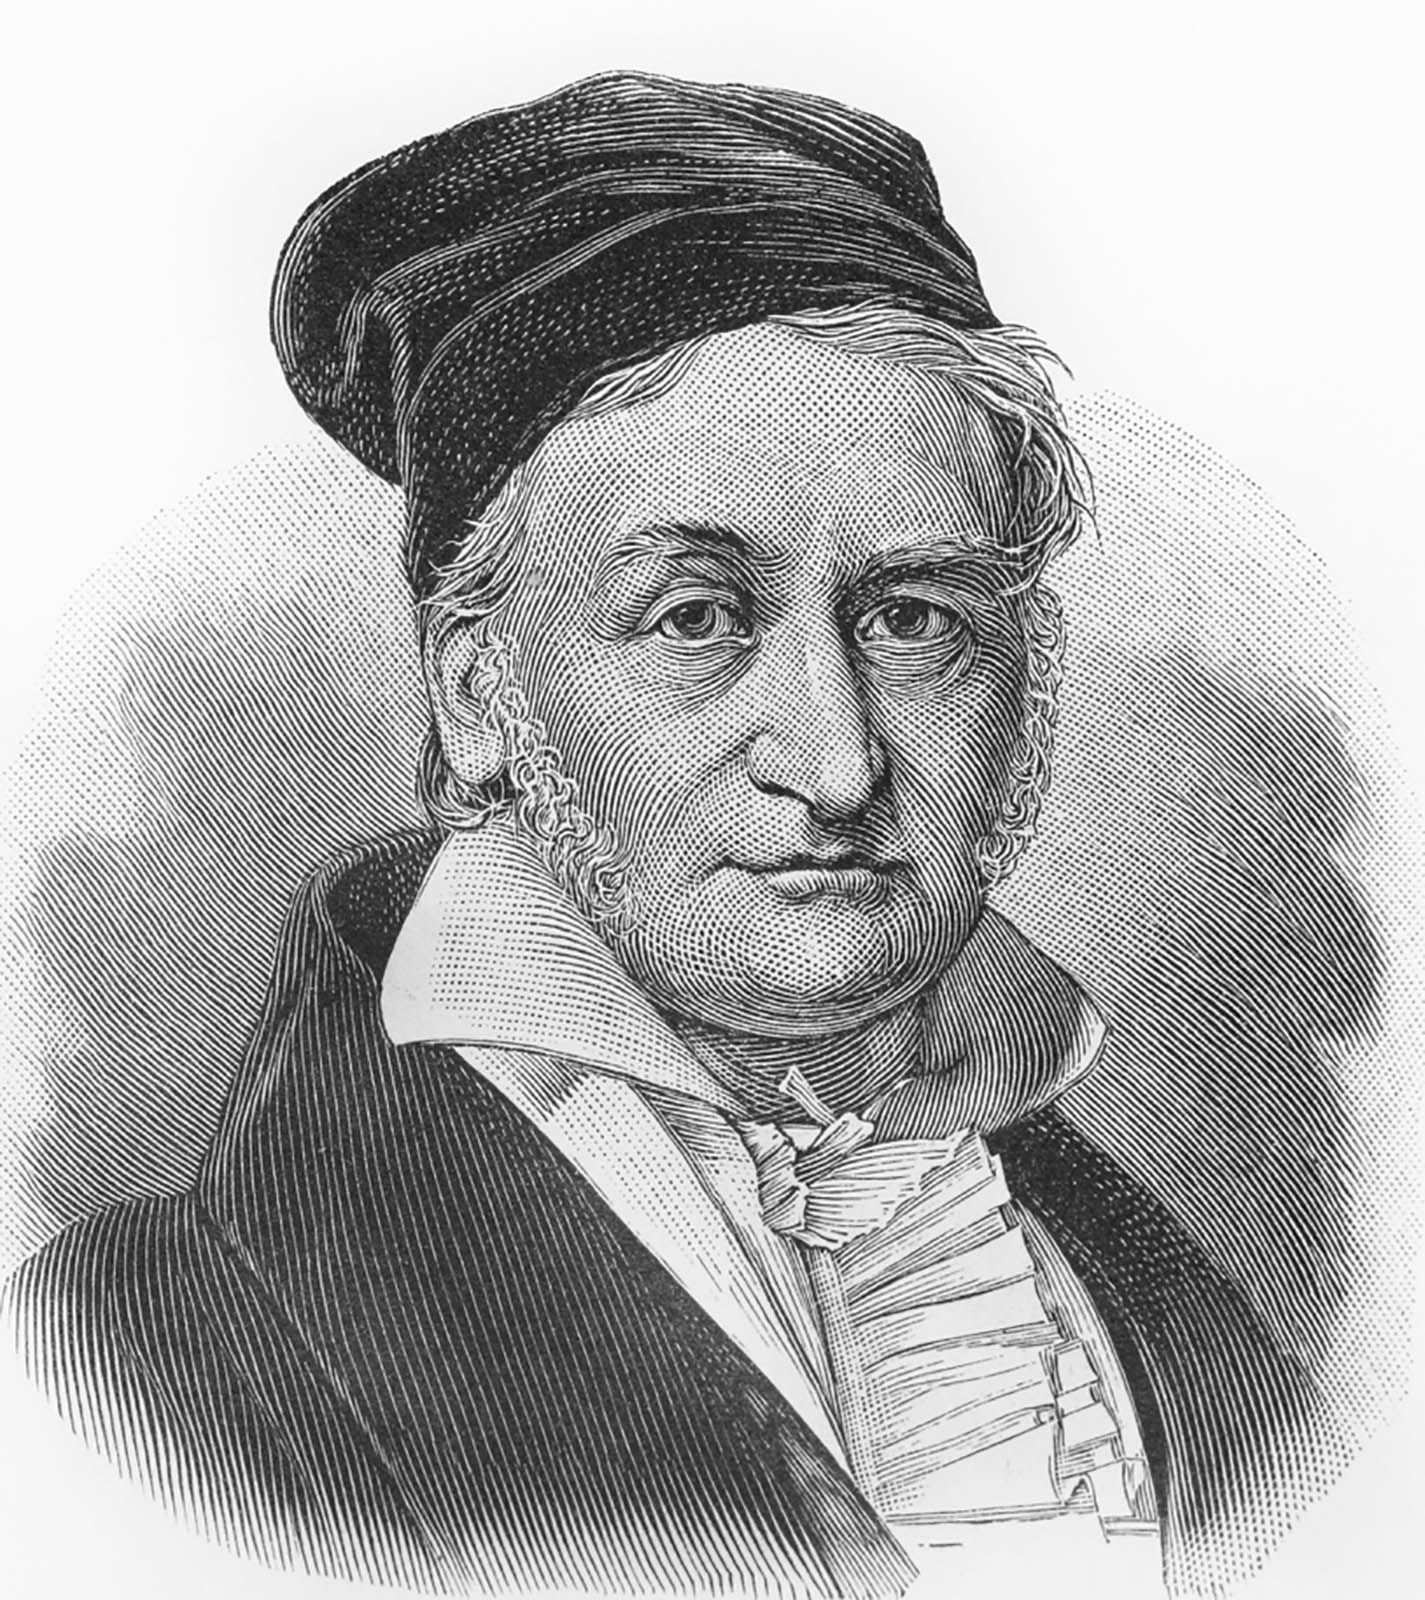
\includegraphics[width=2cm]{Carl-Friedrich-Gauss-engraving.jpg}
\end{wrapfigure}\noindent
Marcelo Papini 
exerceu o magistério no Departamento de Matemática, desde 1982,  após concurso para o cargo de professor auxiliar, sendo aposentado compulsoriamente em 2013. Obeteve o doutoramento no programa de pós-graduação em Ensino, Filosofia e História das Ciências, mantido pela UFBA conjuntamente com a UEFS, com uma \emph{Contribuição ao estudo histórico e crítico do pensamento matemático}.
\end{document}
